\subsection{Findings}
Through the participatory design exercises, we found that the artists were very familiar with Autodesk Maya \cite{MayaSource}. To ease the learning curve, we decided to design the tool with the overall structure of Maya in mind. This doesn't mean that the tool should directly copy how Maya looks and works, but that, when designing the camera tool, we should keep their established mental models \cite{mentalModels} in mind. Since the artists have been working with Maya and other 3D modelling software, they have a certain understanding and expectation of the animation process. As a designer, you create conceptual models for the system. Therefore, it's important to be aware of the users' pre-existing mental models. Another key finding was the fact that most of the artists were working with two computer monitors. This enables them to have the main interface on one monitor, while the other can show secondary windows such as graph editors or an additional preview window showing the camera's point of view.

\subsubsection{Keyframing Concept}
Through ?? of Maya we found that the most important feature from here were keyframes.
A keyframe is an event and/or change in one or more parameters over time. Each keyframe corresponds to a point in time, meaning that when the animation reaches this point in time, the values of this keyframe are dominant. Usually this means that in between keyframes some interpolation is happening. This interpolation is per default linear, but can be manipulated in a graph editor. Anything that can be represented by numbers can be manipulated through keyframes.

But games are dynamic, not linear, so this means keyframes can't be associated with a point in time. Specifically for this game, the camera settings would change according to the player's movement, so keyframes needed to be associated with this. Furthermore, the player had to walk on a fixed path, which made the interpolation significantly simpler.

A quick paper prototype of the initial concept showed promise and the idea of associating keyframes with player position was easily understood. To avoid confusion, these keyframes were renamed \textit{framings}. A framing consists of an \textit{influence point} and a camera (see Figure \ref{fig:framingConcept}). When the player's position is the same as an influence point, that framing will dominate, meaning the main camera will use the camera settings of the associated camera. Moving between influence points causes an interpolation between each camera setting. This interpolation can be manipulated in a graph editor, as in Maya.

\begin{figure}[htbp]
\centering
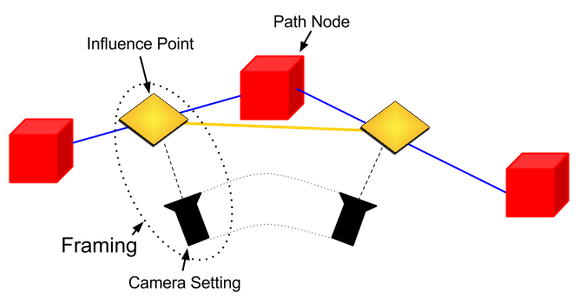
\includegraphics[width=0.4\textwidth]{Pics/Instructions}
\caption{Illustration of the framing concept. A framing consists of an influence point and a group of camera settings.}
\label{fig:framingConcept}
\end{figure}
